\chapter{Characteristics}

\section{Absolute maximum ratings}
Stresses that exceed the limits specified in this section may cause permanent damage to the device. 
Proper operation of the device within the limits specified in this section is not implied.  

\begin{ZubaxTableWrapper}{Absolute maximum ratings}
    \begin{ZubaxWrappedTable}{| X | c | c | c |}
    Parameter                 & Min   & Max    & Unit           \\
    Supply voltage            & -0.3  & 36     &   V            \\
    Phase current amplitude   &       & 45     &   A            \\
    DC continuous current     &       & 30     &   A            \\
    Operating temperature     & -40   & 85     &   \degree{}C   \\
    CAN H/L input voltage     & -0.3  & 7      &   V            \\
\end{ZubaxWrappedTable}
\end{ZubaxTableWrapper}

\section{Environmental conditions}

\begin{ZubaxTableWrapper}{Environmental conditions}
    \begin{ZubaxWrappedTable}{| l | X | c  c | c |}
    Parameter                   & Note                       & Min & Max    & Unit          \\
    Operating temperature       &                            & -40 & 85     & \degree{}C    \\
    Storage temperature         &                            & -40 & 50     & \degree{}C    \\
    Operating humidity          & Condensation not permitted & 0   & 100    & \%RH          \\
    Operating altitude          & Above mean sea level (MSL) &     & 10     & km            \\
\end{ZubaxWrappedTable}
\end{ZubaxTableWrapper}

\section{Operational characteristics}

\begin{ZubaxTableWrapper}{Power characteristics}
\begin{ZubaxWrappedTable}{| l | X | X | c |}\label{table:Power characteristics}
    Parameter                           & Sadulli Piccino   & Sadulli Grosso    & Unit  \\
    Continuous power                    & 500               & 500               &   W   \\
    Peak power (30sec)                  & 700               & 700               &   W   \\
    Thrust in efficient mode\tnote{a}   & 700               & 1500              &   gf  \\
    Max thrust                          & 1500              & 4000              &   gf  \\
\end{ZubaxWrappedTable}
\begin{tablenotes}
\item [a] - The efficient mode is the mode where the device produces not less than 10 gf of thrust per each watt of electrical power consumed
\end{tablenotes}
\end{ZubaxTableWrapper}

\begin{ZubaxSimpleTable}{Mechanical characteristics}{|l|c|c|c|X|}
    Parameter       & Grosso  & Piccino  & Nudo  & Unit & Note                 \\
    Weight          & 228     & 128      & 62    & g    & Cables not included  \\
    IP Protection   & 54      & 54       & 54    & -    & Liquid damage protection is achieved by conformal \mbox{coating} of the PCB \\                        
\end{ZubaxSimpleTable}

\begin{ZubaxTableWrapper}{Characteristics of CAN bus interfaces}
    \begin{ZubaxWrappedTable}{| X |c c c | c |}
        Parameter                                 & Min  & Typ  & Max  & Unit               \\
        Bit rate                                  & 20   &      & 1000 & Kbps               \\
        Positive-going input threshold voltage    &      & 750  & 900  & mV                 \\
        Negative-going input threshold voltage    & 500  & 600  &      & mV                 \\
        Differential output voltage, dominant     & 1.5  & 2.0  & 3.0  & V                  \\
        Differential output voltage, recessive    & -120 & 0    & 12   & mV                 \\
        Bus power rail voltage                    & -10  &      & 10   & V                  \\
        Inter-connector current                   & -1   &      & 1    & A                  \\
        Connector resistance during device lifetime &    & 30   & 50   & $\text{m}\Omega$   \\
    \end{ZubaxWrappedTable}
\end{ZubaxTableWrapper}

\begin{ZubaxTableWrapper}{BEC characteristics}
\begin{ZubaxWrappedTable}{| X | l | c |}
    Parameter            & Value   & Unit               \\
    Output voltage       &  4.9    & V                  \\
    Voltage tolerance    &   2     & \%                 \\
    Maximum load current &  500    & mA                 \\
    Voltage ripple       &  100    & m$V_\text{p-p}$    \\
\end{ZubaxWrappedTable}
\end{ZubaxTableWrapper}

\subsection{Regenerative braking}
During regenerative braking, the device performs energy transfer from the motor to the power supply network. 
If the self-resistance of the power supply network is not sufficiently low, 
the regenerative energy transfer may lead to an increase of the supply voltage beyond the safe operating limits. 
Generally, batteries are capable of absorbing the energy recovered during braking without issues. 
Problems may arise if the device is powered from a source that does not permit high reverse currents, 
such as laboratory power supplies. 
In that case, it is advised to install additional buffer capacitors to act as energy storage during braking.

\subsection{Power connectors}
Zubax Sadulli is equipped with an XT30PW-M power connector. 
The mating XT30U-F connector may be provided as connector only or as a connector with pre-soldered 100 mm 16 AWG wires.

\section{CAN bus}

The device is equipped with a single ISO 11898-2 CAN 2.0A/B interface. 
CAN interface has two standard UAVCAN Micro connectors\footnote{Refer to \url{http://uavcan.org} for more information on UAVCAN.} 
joined in parallel. The device does not terminate the CAN bus internally.

\begin{ZubaxSimpleTable}{CAN bus connectors pinout}{| c | X | X | }
    Pin no. & Type         & Name   \\   
    1       & Power        & PWR    \\  
    2       & Input/Output & CAN H  \\  
    3       & Input/Output & CAN L  \\  
    4       & Ground       & GND    \\
\end{ZubaxSimpleTable}

\section{BEC output}
Zubax Sadulli features software-controllable BEC output. It is available on bus power supply pin of UAVCAN connectors. 
BEC output is protected against short circuit, maximum output current is 500 mA.  
It is also protected against the reverse current flow with an ideal diode. 

\newpage

\section{Indication}

\newcommand{\LEDX}{{\rule{0.4em}{1.0em}}}
\newcommand{\LEDO}{{\rule{0.4em}{0.1em}}}
\newcommand{\ShowColor}[1]{{\color{#1}\rule{2em}{0.8em}}}

Zubax Sadulli is equipped with two separate LED indicators that reflect its status.

\textbf{CAN} green LED indicates data transfer through the CAN bus. 
Blinks once if at least one CAN frame was successfully transmitted or successfully received in the last 25 milliseconds. 
Glows steadily when the intensity of CAN traffic is higher than 40 frames per second.

\textbf{STATUS} RGB LED indicates the status of the firmware. 
The behaviour of the status LED is specified in the table below.

\begin{ZubaxSimpleTable}{Status LED during boot}{|l l X|}\label{table:status_led}
             Color              & Status                              & Description                                  \\
    \ShowColor{yellow} Yellow   & No application to boot              & The firmware has not been flashed to the ESC
                                                                        or FLASH has been damaged.                   \\
    \ShowColor{blue} Blue       & Application upgrade is in progress  &                                              \\
    \ShowColor{green} Green     & Boot canceled                       & The device firmware has not been properly signed \\
    \ShowColor{magenta} Magenta & Ready to boot                       & Glows after the device power-up or restart event
                                                                        until the application starts. \\
\end{ZubaxSimpleTable}

\begin{ZubaxSimpleTable}{Status LED behavior}{|l X X|}\label{table:status_led_behavior}
    LED pattern (step 80 ms)                     & Status                    & Description\\

    {\color{blue}
       \LEDX\LEDO\LEDO\LEDO\LEDO\LEDX}           & Idle, ready to run        & The ESC is ready and waiting for the
                                                                               setpoint.\\
    
    {\color{red}
       \LEDX\LEDO\LEDO\LEDO\LEDO\LEDX\LEDX\LEDX} & Idle, hardware fault      & The power stage is not ready or current
                                                                               is tripped.\\

    {\color{red}
       \LEDX\LEDO\LEDO\LEDO\LEDO\LEDX\LEDO\LEDX\LEDX\LEDX}
                                                 & Idle, hardware test fault & The motor is not connected or there is a
                                                                               short circuit on the output of the
                                                                               ESC.\\

    {\color{red}
       \LEDX\LEDO\LEDO\LEDO\LEDO\LEDX\LEDO\LEDX\LEDO\LEDX\LEDO\LEDX\LEDO\LEDX\LEDO\LEDX\LEDO\LEDX\LEDX\LEDX\LEDO\LEDX
       \LEDX\LEDX}                          & Idle, invalid motor parameters & Some motor parameters are not properly
                                                                               initialized or the motor identification
                                                                               hasn't been performed.\\
\end{ZubaxSimpleTable}

\newpage

\section{Mechanical characteristics}

The drawing \ref{connecotrs} documents the placement of connectors and status LEDs on all variants of Zubax Sadulli.

\begin{figure}[!hbt]
    \centerline{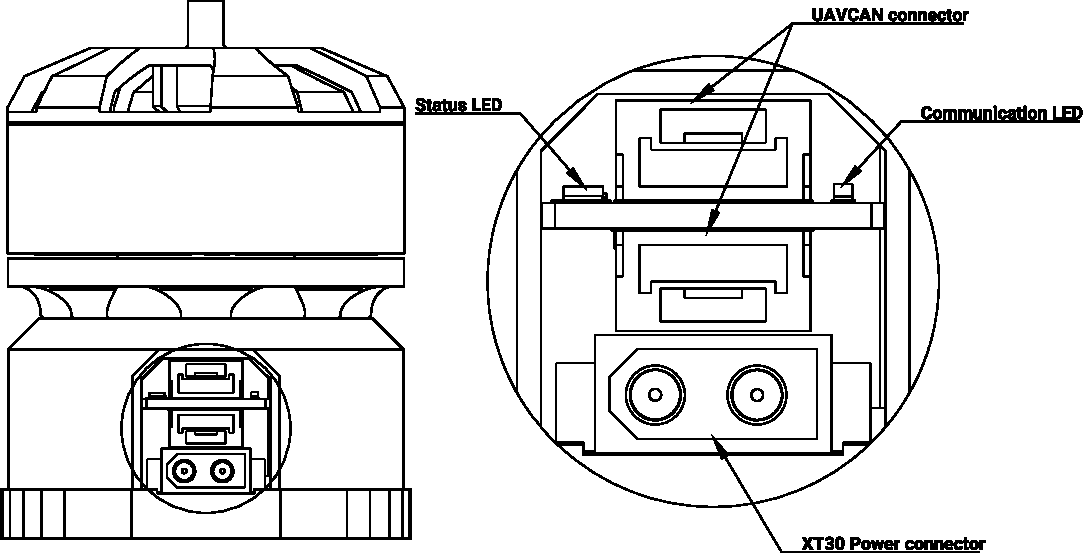
\includegraphics[width=0.8\textwidth]{figures/connectors_leds}}
    \caption{Connectors and LEDs drawing\label{connecotrs}}
\end{figure}

\subsection{Mounting pattern}

All versions of Zubax Sadulli share the same mounting pattern. 
It is specified in the drawing \ref{mounting_pattern} All linear dimensions are in mm.

\begin{figure}[!hbt]
    \centerline{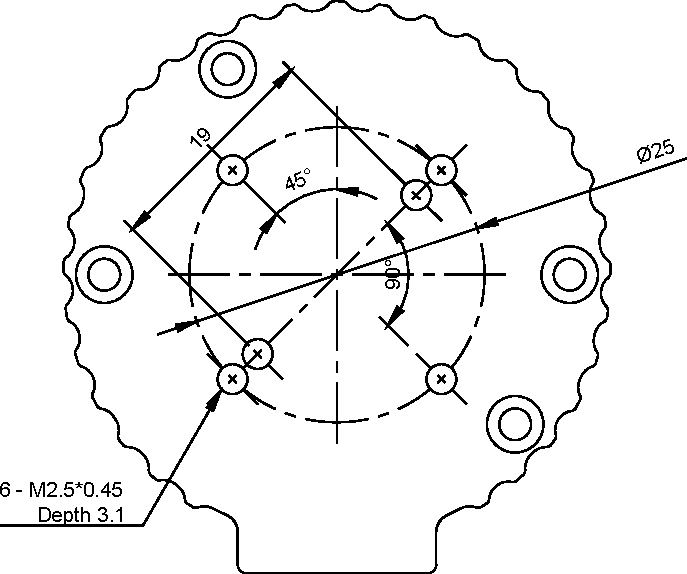
\includegraphics[width=0.7\textwidth]{figures/mounting_pattern}}
    \caption{Mounting pattern\label{mounting_pattern}}
\end{figure}

\newpage

\subsection{Sadulli nudo drawing}
All linear dimensions are in mm.

\begin{figure}[!hbt]
    \centerline{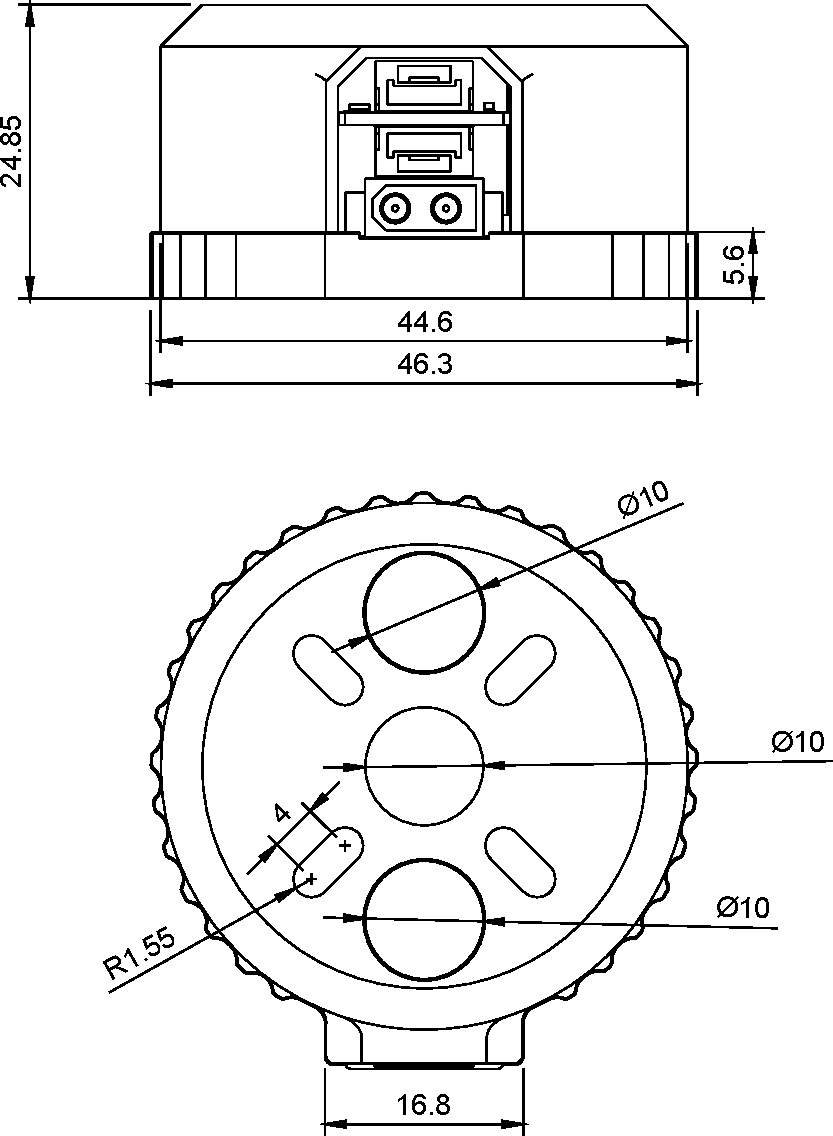
\includegraphics[width=0.8\textwidth]{figures/sadulli_nudo}}
    \caption{Sadulli Nudo drawing\label{Nudo_drawing}}
\end{figure}

\newpage

\subsection{Sadulli Piccino drawing}
All linear dimensions are in mm. Propeller not shown.

\begin{figure}[!hbt]
    \centerline{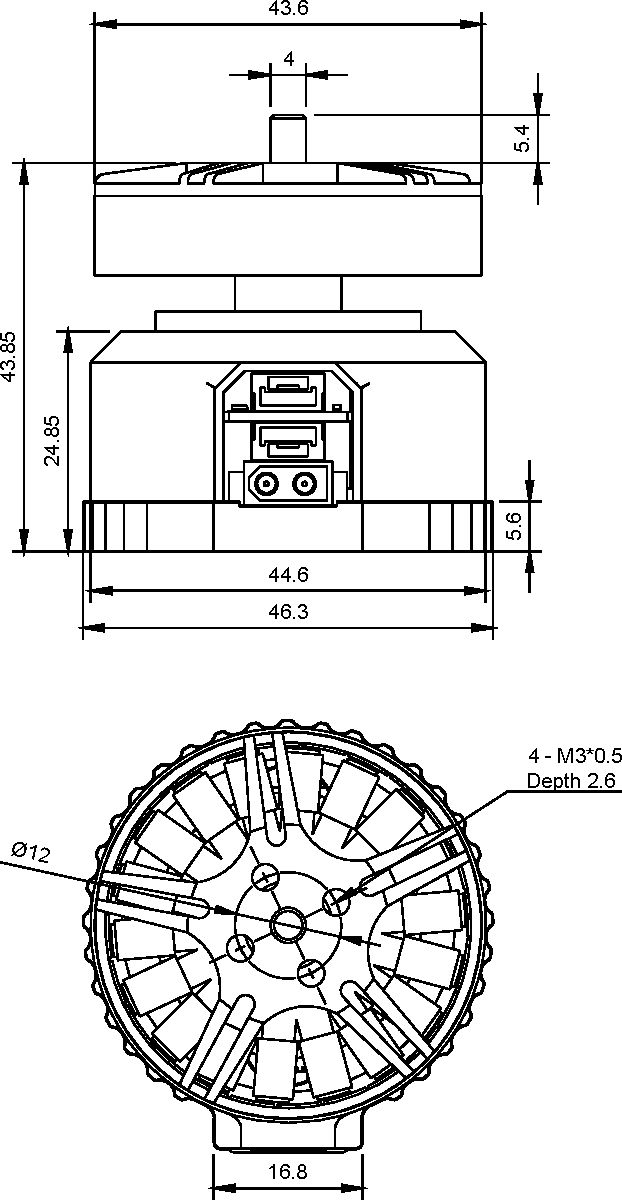
\includegraphics[width=0.6\textwidth]{figures/sadulli_piccino}}
    \caption{Sadulli Piccino drawing\label{Piccino_drawing}}
\end{figure}

\newpage

\subsection{Sadulli Grosso drawing}
All linear dimensions are in mm. Propeller not shown.

\begin{figure}[!hbt]
    \centerline{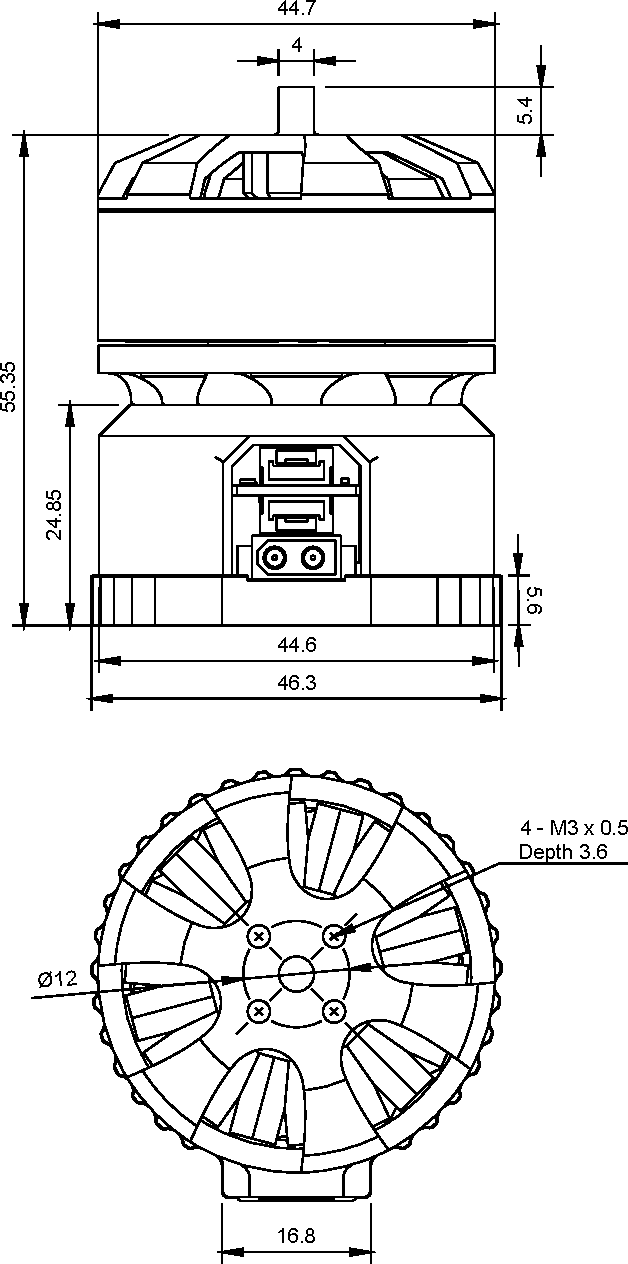
\includegraphics[width=0.6\textwidth]{figures/sadulli_grosso}}
    \caption{Sadulli Grosso drawing\label{Grosso_drawing}}
\end{figure}
